\documentclass{article}

\usepackage{tikz}

 

\begin{document}

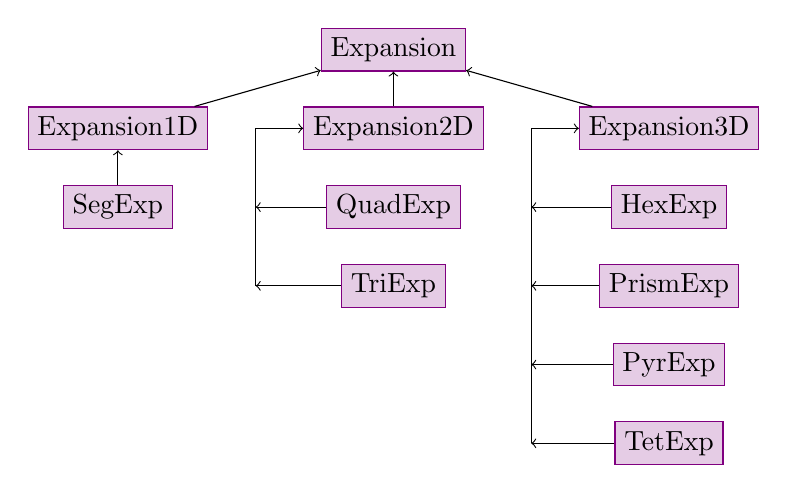
\begin{tikzpicture}[outline/.style={draw=#1,fill=#1!20}]

%NODES


\node [outline= violet] (Expansion)                                   at (3.5,0)          {Expansion};

\node [outline= violet] (Expansion1D)                              at (0,-1)        {Expansion1D};
\node [outline= violet] (Expansion2D)                              at (3.5,-1)        {Expansion2D};
\node [outline=violet] (Expansion3D)                              at (7,-1)        {Expansion3D};

\node [outline=violet] (SegExp)                    at (0,-2)         {SegExp};
\node [outline=violet] (QuadExp)                    at (3.5,-2)         {QuadExp};
\node [outline=violet] (TriExp)                    at (3.5,-3)         {TriExp};
\node [outline= violet] (HexExp)                    at (7,-2)         {HexExp};
\node [outline= violet] (PrismExp)                    at (7,-3)         {PrismExp};
\node [outline=violet] (PyrExp)                    at (7,-4)         {PyrExp};
\node [outline=violet] (TetExp)                    at (7,-5)         {TetExp};




%CONNECTIONS


\draw[<-] (Expansion2D)--(1.75,-1);

\draw (1.75,-2) -- (1.75,-1) ;
\draw[<-] (1.75,-2)--(QuadExp);

\draw (1.75,-3) -- (1.75,-2) ;
\draw[<-] (1.75,-3)--(TriExp);

\draw[<-] (Expansion3D)--(5.25,-1);

\draw (5.25,-2) -- (5.25,-1) ;
\draw[<-] (5.25,-2)--(HexExp);

\draw (5.25,-3) -- (5.25,-2) ;
\draw[<-] (5.25,-3)--(PrismExp);

\draw (5.25,-4) -- (5.25,-3) ;
\draw[<-] (5.25,-4)--(PyrExp);

\draw (5.25,-5) -- (5.25,-4) ;
\draw[<-] (5.25,-5)--(TetExp);

%\draw[->] (8,-4)--(8,0);
%\draw[->](ExpListHomogeneous1D)--(8,-4);

\path[<-]  (Expansion)      edge (Expansion1D)
                 (Expansion)      edge (Expansion2D)
                 (Expansion)      edge (Expansion3D)
                 (Expansion1D)      edge (SegExp);

\end{tikzpicture}


\end{document}